% !TeX root = ../beamer.tex
\section{Beleuchtungsquellen}

\begin{frame}
  \frametitle{Beleuchtungsquellen (Illuminators of Opportunity)}

  \begin{columns}
    \begin{column}{0.2\textwidth}
      \begin{figure}
        \raggedleft{}
        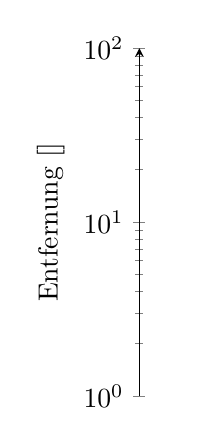
\begin{tikzpicture}
          \begin{axis}[
              ymode=log,
              height=6cm,
              width=2cm,
              hide x axis,
              axis y line=left,
              ymin=1,
              ymax=100,
              ylabel={Entfernung [\si{\kilo\metre}]},
            ]
            \addplot [draw=none] {1};
          \end{axis}
        \end{tikzpicture}
      \end{figure}
    \end{column}
    \begin{column}{0.8\textwidth}
      \begin{itemize}
        \item FM-Radio
        \item DVB-T (Digitales Fernsehen)
        \item DAB (Digitales Radio)
        \item LTE
        \item GSM
        \item WiFi
      \end{itemize}
    \end{column}
  \end{columns}
\end{frame}
